\begin{figure}[t]
\centering
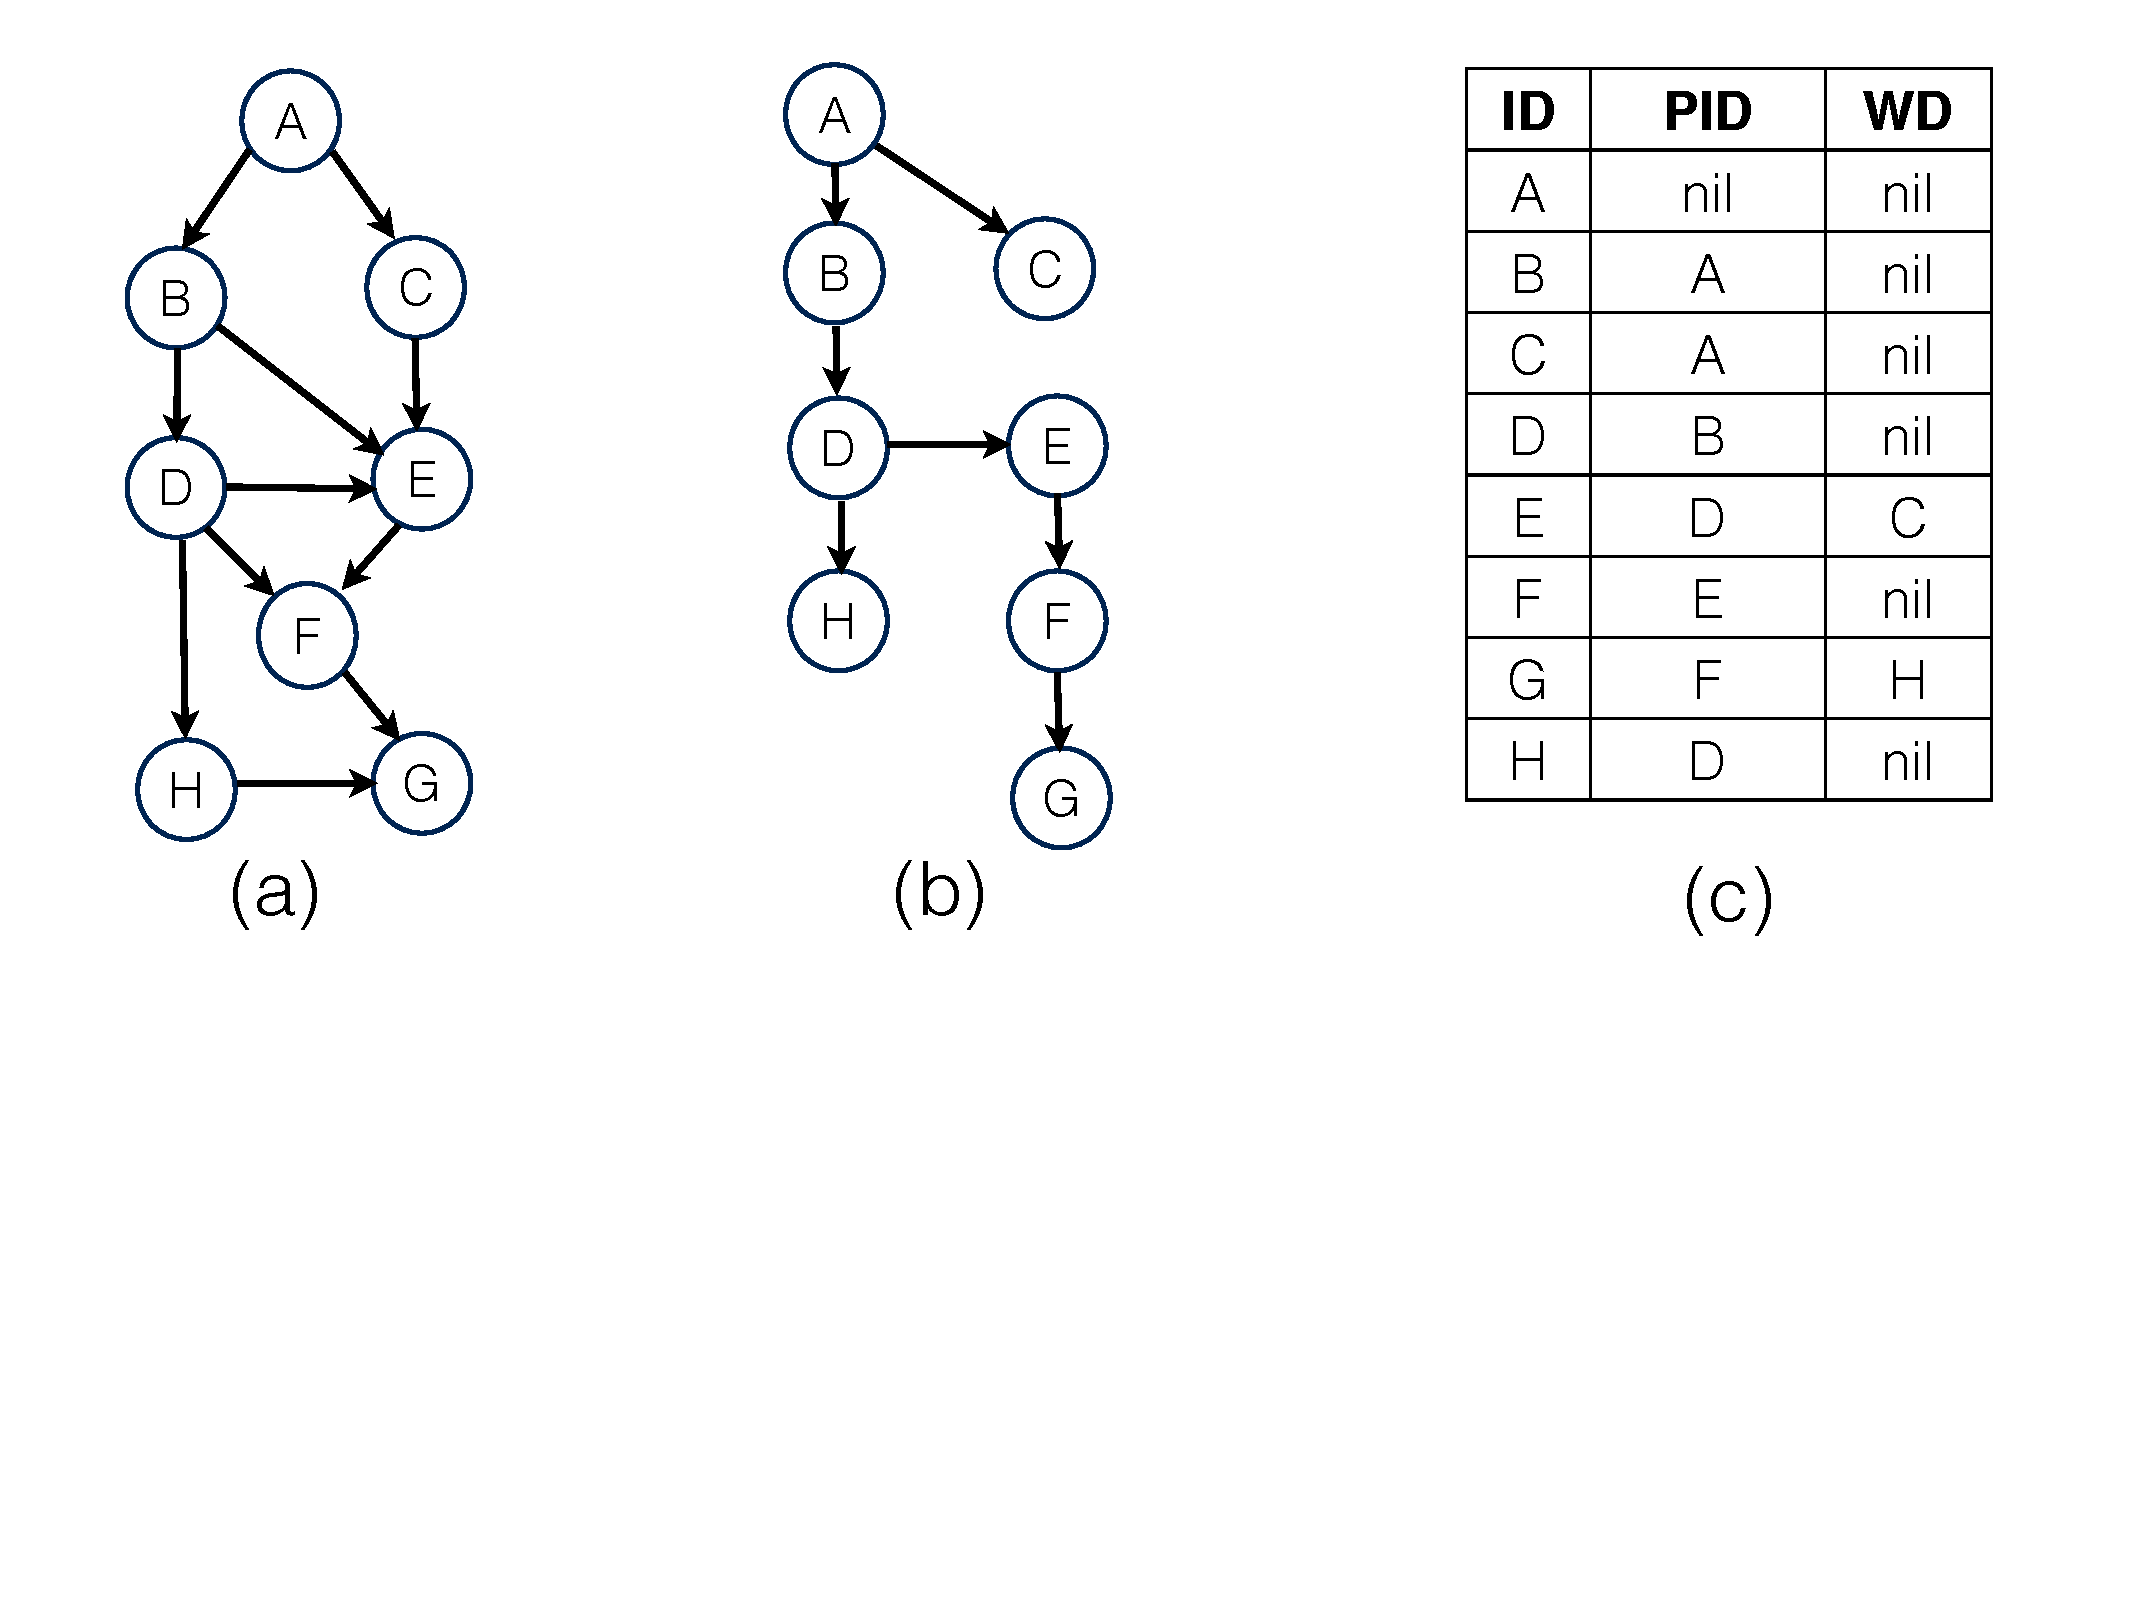
\includegraphics[width=0.8\textwidth]{chapter3/di_indexing.pdf}
	\caption{I-Index Construction over the Pathway DAG in Figure~\ref{fig:topological}. (a) shows the DAG structure; (b) provides the inheritance relationship discovered during the index construction; (c) shows the final I-Index.}
	\label{fig:diff-index}
\end{figure}

\section{Inheritance Index}
\textit{DBIndex} is a general index that can support both k-hop as well as
topological window queries. 
%This is intuitive as the window matrix is able to cover both k-hop window or topological window. 
However, the evaluation of a topological window function, $W_t$, 
can be further optimized due to its containment feature. 
In other words, the window of a descendant vertex 
completely covers that of one of its ancestors. 
This feature can be formally formulated in the following theorem. 

\begin{theorem}
\label{thm:containment}
In a DAG, if vertex u is the ancestor of vertex v, the topological window of $v$, $W_t(v)$ completely contains the window of $u$, $W_t(u)$, i.e., $W_t(u) \subset W_t(v)$.   
\end{theorem}

\begin{proof}
In a DAG, if $u$ is the ancestor of $v$, then $u \leadsto v$. $\forall w \in W_t(u)$, then $w \leadsto u$. As $u \leadsto v$, then $w \leadsto v$. Thus, $w \in W_t(v)$ and the theorem is proved.   
\end{proof}

Let us consider the BioPathway graph in Figure~\ref{fig:topological} as
an example.
Figure~\ref{fig:diff-index} (a) shows its abstract DAG. In (a), 
D is the ancestor of E. In addition, we can see that the window of $D$, 
$W_t(D)$ is $\{A, B, D\}$ and the window of $E$, $W_t(E)$ is $\{A, B, D, C, E\}$. It is easy to see that $W_t(D) \subset W_t(E)$. 

Now, Theorem~\ref{thm:containment} provides us with opportunities for optimizing
the space and computation of topological window queries. 
First, since the set of vertices corresponding to the
window of a node, say $u$, is a superset of the set of vertices of its
parent node, say $v$, there is no need to maintain the full set of 
vertices of the window at $u$. Instead, 
we only need to maintain the difference between 
$W_t(u)$ and $W_t(v)$. We note that in a DAG, it is possible for $u$ to have
multiple parents, $v_1, \cdots, v_k$. In this case, the parent
which has the smallest difference with $u$ can be used; where there
is a tie, it is arbitrarily broken.
We refer to this parent as the {\em closest} parent. For instance, in Figure~\ref{fig:diff-index} (a), instead of maintaining 
$\{A, B, D, C\}$ for $W_t(E)$, it can simply maintain the difference 
to $W_t(D)$ which is $\{C\}$. This is clearly more space efficient.

Second, using a similar logic, the aggregate computation
at a node $u$ can actually reuse the 
aggregate result of its closest parent, $v$.
Referring to our example, the aggregation result of $W_t(D)$ can be 
simply passed or inherited to $W_t(E)$ and further aggregated with the difference 
set ($\{C\}$) in $W_t(E)$ to generate the aggregate value for $W_t(E)$. 
Figure~\ref{fig:diff-index} (b) indicates the inheritance relationship that 
the values of the father can be inherited to the child in the tree. 

Thus, we propose a new structure, called the \textbf{inheritance index}, 
$I$-$Index$, to support efficient processing of topological window queries. 
In $I$-$Index$, each vertex $v$ maintains two information. 
\begin{itemize}
\item The first information is the ID of the closest parent (say $u$) 
of $v$. We denote this as PID($v$).
\item The second information is the difference between 
$W_t(v)$ and $W_t(u)$. We denote this as WD($v$). 
\end{itemize}

With PID($v$), we can retrieve $W_t(u)$, and combining with 
WD($v$), we can derive $W_t(v)$. 
Likewise, we can retrieve the aggregation result of $u$ 
which can be reused to compute $v$'s aggregation result.

Figure~\ref{fig:diff-index}(c) shows the I-index of our example
in Figure~\ref{fig:diff-index}(a). In the figure, I-Index
is represented in a table format; 
the second column is the PID and the third indicates the WD. 

\subsection{Index Construction} 

Building an I-Index for a DAG
can be done efficiently. 
This is because the containment relationship can be easily 
discovered using a topological scan.
Algorithm~\ref{algo:piconstruction} lists the pseudo code for 
index creation. 
The scheme iterates through all the vertices in a topological order.
For vertex $v$, the processing involves two steps.
In the first step, we determine the closest parent
of $v$. This is done by comparing the cardinalities of 
the windows of $v$'s parents, and 
find the parent with largest value. 
The corresponding PID is recorded in the \emph{PID} field of 
I-Index (Lines~\ref{algo:tp-step1-start}-\ref{algo:tp-step1-stop}). 
In the second step, the window of $v$, $W_t(v)$, is pushed to 
its children 
(Lines~\ref{algo:tp-step2-start}-\ref{algo:tp-step2-stop}). 
When the processing of $v$ finishes, its window can be discarded. This
frees up the memory space, which makes the scheme memory efficient.

We not that the complexity of Algorithm~\ref{algo:piconstruction} is non-trivial to analyze. 
This dues to the difficulty of analyzing of the number of ancestors of each vertex. Suppose the 
average number of ancestors for each vertex is $H$, then Algorithm~\ref{algo:piconstruction} is of
complexity $O(H|V|*d)$, where $d$ is the average degree of the graph. This complexity is close to the
output complexity. That is to gather the all vertex-window mapping, at least $O(H|V|)$ elements needs
to be outputted. Thus the indexing time complexity is reasonably efficient.

We further note that the size of \emph{I-Index} is hard to be precisely evaluated. 
This dues to the difficulty of analyzing the window difference. Assume the average size of window difference
is $D$, then the size of \emph{I-Index} is $O(D|V|)$. Although $D$ can be as large $O(|V|)$, our 
experimental results indicate that the index size is always 
comparable to the graph size. We defer this discussion to 
section \ref{sec:experiments}. Furthermore, it is possible to
reduce the index size (should it be a concern) by employing
compression techniques. 

\begin{algorithm}[h]
\label{alg:piconstruction}
\caption{CreateI-Index}
\begin{algorithmic}[1]
\Require Input graph: $G$ 
\Ensure Inheritance Index: $IIndex$ 
\State $IIndex \leftarrow ()$
\State $p \leftarrow ()$ \Comment{stores the window for each vertex}
\State $c \leftarrow ()$ \Comment{stores the cardinality of window for each vertex}
\ForAll{$v \in$ topological order}
\State $WD \leftarrow -\infty$ \Comment{the window difference}
\State $bestu \leftarrow nil$
\ForAll{$u \in v.parent$} \label{algo:tp-step1-start}
	\If{$c[u] > diff$} 
		\State $diff \leftarrow c[u]$
		\State $bestu \leftarrow u$
	\EndIf
\EndFor \label{algo:tp-step1-stop}
\State $IIndex[v].WD \leftarrow WD$
\State $IIndex[v].PID \leftarrow bestu$
\State $p[v] \leftarrow p[v] \cup v$
\ForAll{$u \in v.child$} \label{algo:tp-step2-start}
	\State $p[u] \leftarrow p[u] \cup p[v]$
\EndFor \label{algo:tp-step2-stop}
\State $c[v] \leftarrow |p[v]|$ \Comment{update window cardinality}
\State $p[v] \leftarrow ()$ \Comment{release memory}
\EndFor
\end{algorithmic}
\label{algo:piconstruction}
\end{algorithm}

%In our experiments, we have evaluated various datasets. 
%The experimental results indicate that the index size is always 
%comparable to the graph size. We defer this discussion to 
%section \ref{sec:experiments}. Furthermore, it is possible to
%reduce the index size (should it be a concern) by employing
%compression techniques. 


\subsection{Query Processing using I-Index}

By employing the I-Index, window aggregation can be processed efficiently 
for each vertex according to 
the topological order. Algorithm \ref{alg:dstw-index} 
provides the pseudo code for the query processing. 
Each vertex $v$'s window aggregation value can be calculated 
by using the following formula: 
\begin{equation}
\Sigma (W_t(v)) = \Sigma (W_t(v.PID),\Sigma(v.WD))
\end{equation}
%%% TANKL: this doesn't work for average!! or min or max!!!
%%%%
where $\Sigma$ is the aggregate function. As the vertex is 
processed according to the topological order, $W_t(v.PID)$ 
would have already been calculated while processing $v$'s parent and 
thus can be directly used for $v$ without any recompution. 
In general, $v$'s window aggregation is achieved by utilizing its 
parent's aggregate value and window difference sets. 
This avoids repeated aggregate computation and achieves 
the goal of computation sharing between a vertex and its parent. 
In so doing, the computation overhead can be further reduced. 
Take the index  provided in Figure~\ref{fig:diff-index} (c) as an example, 
assume the query wants to calculate the sum value over each window 
for every vertex. As a comparison, the number of add operations 
are 33, 22, 16 for the cases without any index, 
with DBIndex and with I-Index index respectively. 


\begin{algorithm}
\caption{QueryProcessingOverIIndex}
\begin{algorithmic}[1]
\Require Input graph $G$, aggregate function $\Sigma$, inheritance index $IIndex$ 
\Ensure $w$ \Comment{The aggregation result of each vertex}
\State $w \leftarrow ()$
\ForAll{$v \in$ topological order} \label{code:dstw-index-tp1}
	\State $u \leftarrow IIndex[v].PID$
	\State $WD \leftarrow IIndex[w].WD$
	\State $S \leftarrow v.val$
	\State $S \leftarrow \Sigma(S, w[u])$
	\ForAll{$t \in WD$ } \label{code:dstw-index-tp2}
		\State $S\leftarrow \Sigma(S, t.val)$
	\EndFor
	\State $w[v] \leftarrow S$
\EndFor
\Return $w$
\end{algorithmic}
\label{alg:dstw-index}
\end{algorithm}

As the query processing in Algorithm~\ref{alg:dstw-index} basically scans the \emph{I-Index}, the query
complexity essentially correlates to the index size. As we shown in the experiment session, the query can be performed efficiently 
in various graph conditions. We defer the discussion to Section 6.


\subsection{Handling Updates}
%\remark{
%Similar to DBIndex, attribute updates on I-Index is easy, since I-Index is built on the structure of the graph.
%The general idea for handling structural updates is to identify the region that affected by the structure updates. Because adding or deleting an isolated node is trivial, the core part of structure update is adding/deleting edges. We observe that the region that affected by inserting/deletion edge $e(u,v)$ can be bounded by the subgraph between \emph{Lowest Common Ancestor} of $u,v$ and $v$. Since we do not focus on dynamic graph, we omit the detail here. Interested user may refer to the extended report of this paper \cite{}.}
%\eat{
We cover the updates handling in this section. For attribute updates, \emph{I-Index} is not affected since \emph{I-Index} is only structure related. Structure updates on \emph{I-Index} consists of node updates and edge updates. It is easy to handle the case where an isolated node is added or delete, since it does not affect any other nodes in the graph. Adding (resp. deleting) a node with edges can be done via edge insertions (resp. deletions). Here we focus on describing single edge insertion and deletion. We use $I$ to denote the \emph{I-index} and $I(v)$ to denote the index entry of $v$. 

During an update of edge $e(s,t)$, there are two types of vertices are affected. The first type contains single node $t$, which is the endpoint of edge $e$. The second type of nodes contains all the descendants of $t$. There are altogether four special cases needs to be consider during the updates. We illustrate the four cases with aids of Figure~\ref{fig:dag_update}. In Figure~\ref{fig:dag_update}, the dashed edge $e(s,t)$ is the edge to be updated (added or deleted). The node $u$ is the \emph{lowest common ancestor}(LCA) of $t$ and $s$. The cloud shape $A$ and $B$ are nodes in between of $u,s$ and $u,t$. Since $u$ is the \emph{LCA}, $A$ and $B$ are thus disjoint. Bold edge $e(c,d)$ indicate that $I(d).PID$ is $c$. We distinguish and handle the four cases as follows:

\textbf{Case I ($I(t).PID = s$)}: As shown in Figure~\ref{fig:dag_update} (a), during deletion, $t$ needs to choose a parent from $A$ to be its $I(t).PID$. $I(t).WD$ needs to be updated accordingly. In this case, no insertion needs to be considered since if there is no edge between $s$ and $t$, $I(t).PID$ cannot be $s$. 

\textbf{Case II ($I(t).PID \neq s$)}: As shown in Figure~\ref{fig:dag_update} (b), during insertion, $B$ needs to be excluded from $I(t).WD$. During deletion, any node in $B$ that cannot reach $t$ needs to be included in $I(t).WD$. Since $A$ and $B$ are disjoint, every node in $B$ needs to be removed from $I(t).WD$

\textbf{Case III ($t \leadsto I(v).PID$)}: As shown in Figure~\ref{fig:dag_update} (c), during insertion, any node in $B$ needs to be removed from $I(v).WD$. During deletion, any node in $B$ that reaches $v$ but cannot reach $a$ needs to be added to $I(v).WD$.

\textbf{Case IV ($t \nrightarrow I(v).PID$)}: As shown in Figure~\ref{fig:dag_update} (d), during insertion, any node in $B$ that cannot reach $r$ needs to be included into $I(v).WD$. During deletion, any node in $B$ that cannot reach $v$ needs to be excluded from $I(v).WD$.

During structure updates, essential operations are computing $A,B$ and performing reachability queries. Computing $A,B$ can be done via existing techniques such as \cite{bender2005lowest,czumaj2007faster} while reachability query can be supported by indexing methods such as \cite{yildirim2013dagger}. We defer exploring for more efficient updating algorithms to future work 


\begin{figure*}[t]
\centering
\begin{subfigure}{0.22\linewidth}
  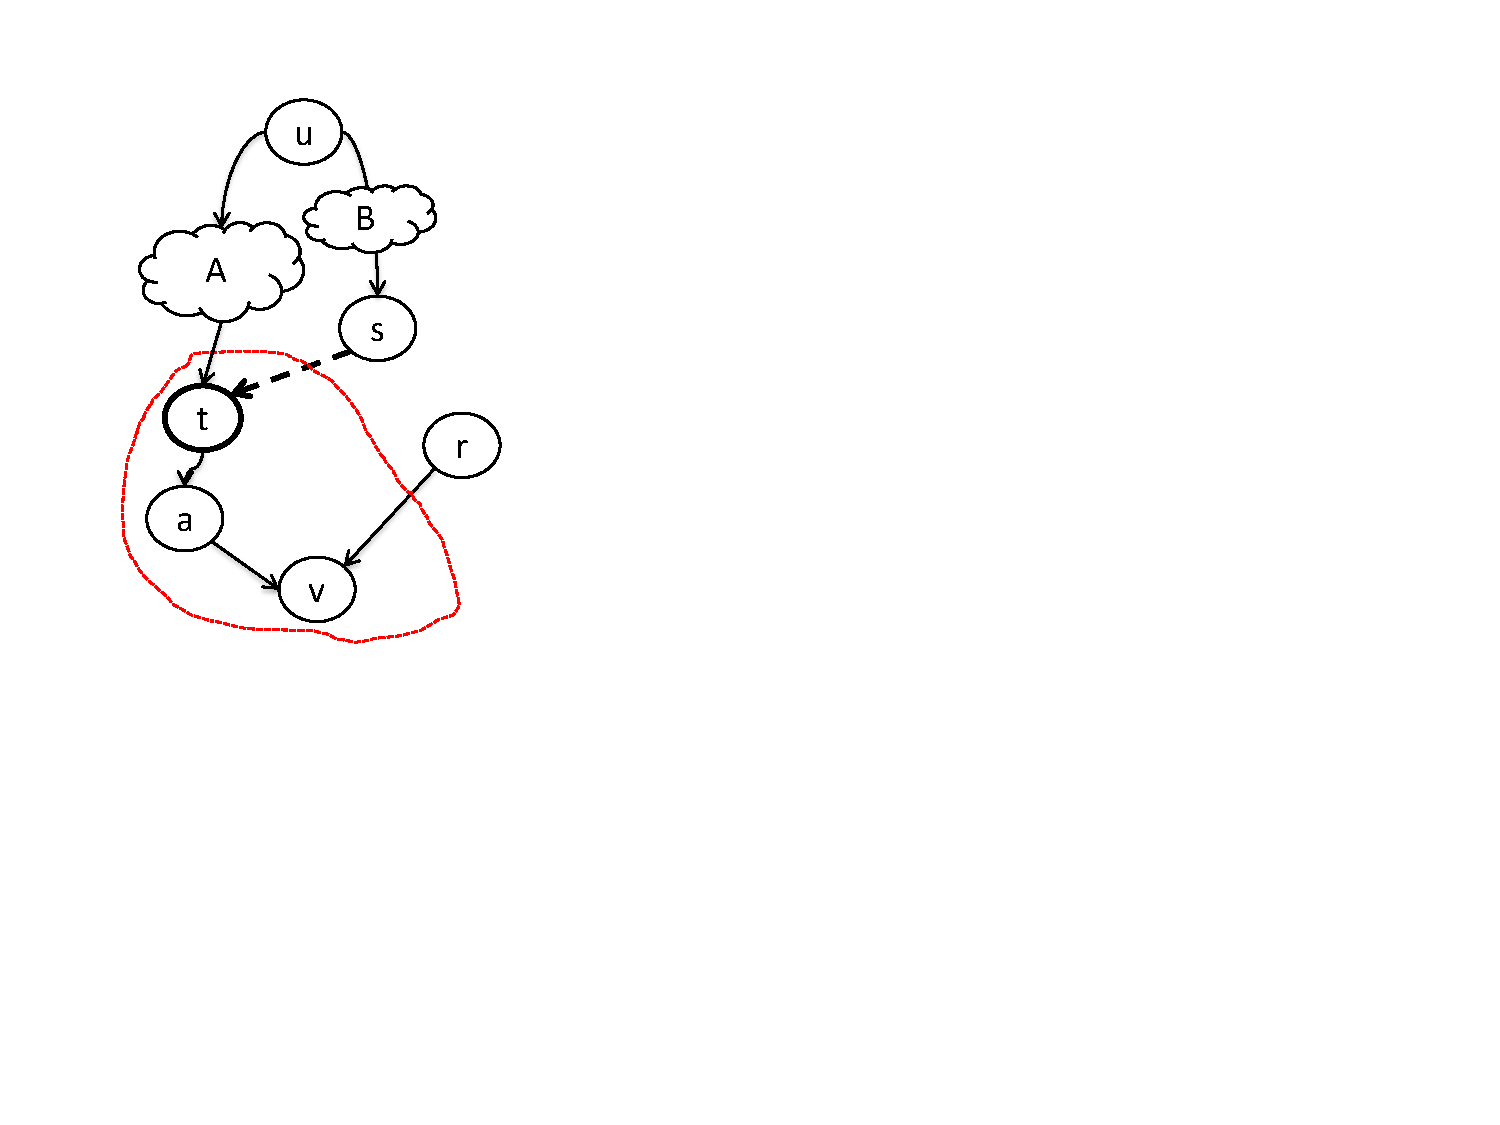
\includegraphics[width=\textwidth]{chapter3/dag_update_1.pdf}
  \caption{Case 1}
\end{subfigure}%
\begin{subfigure}{0.22\linewidth}
  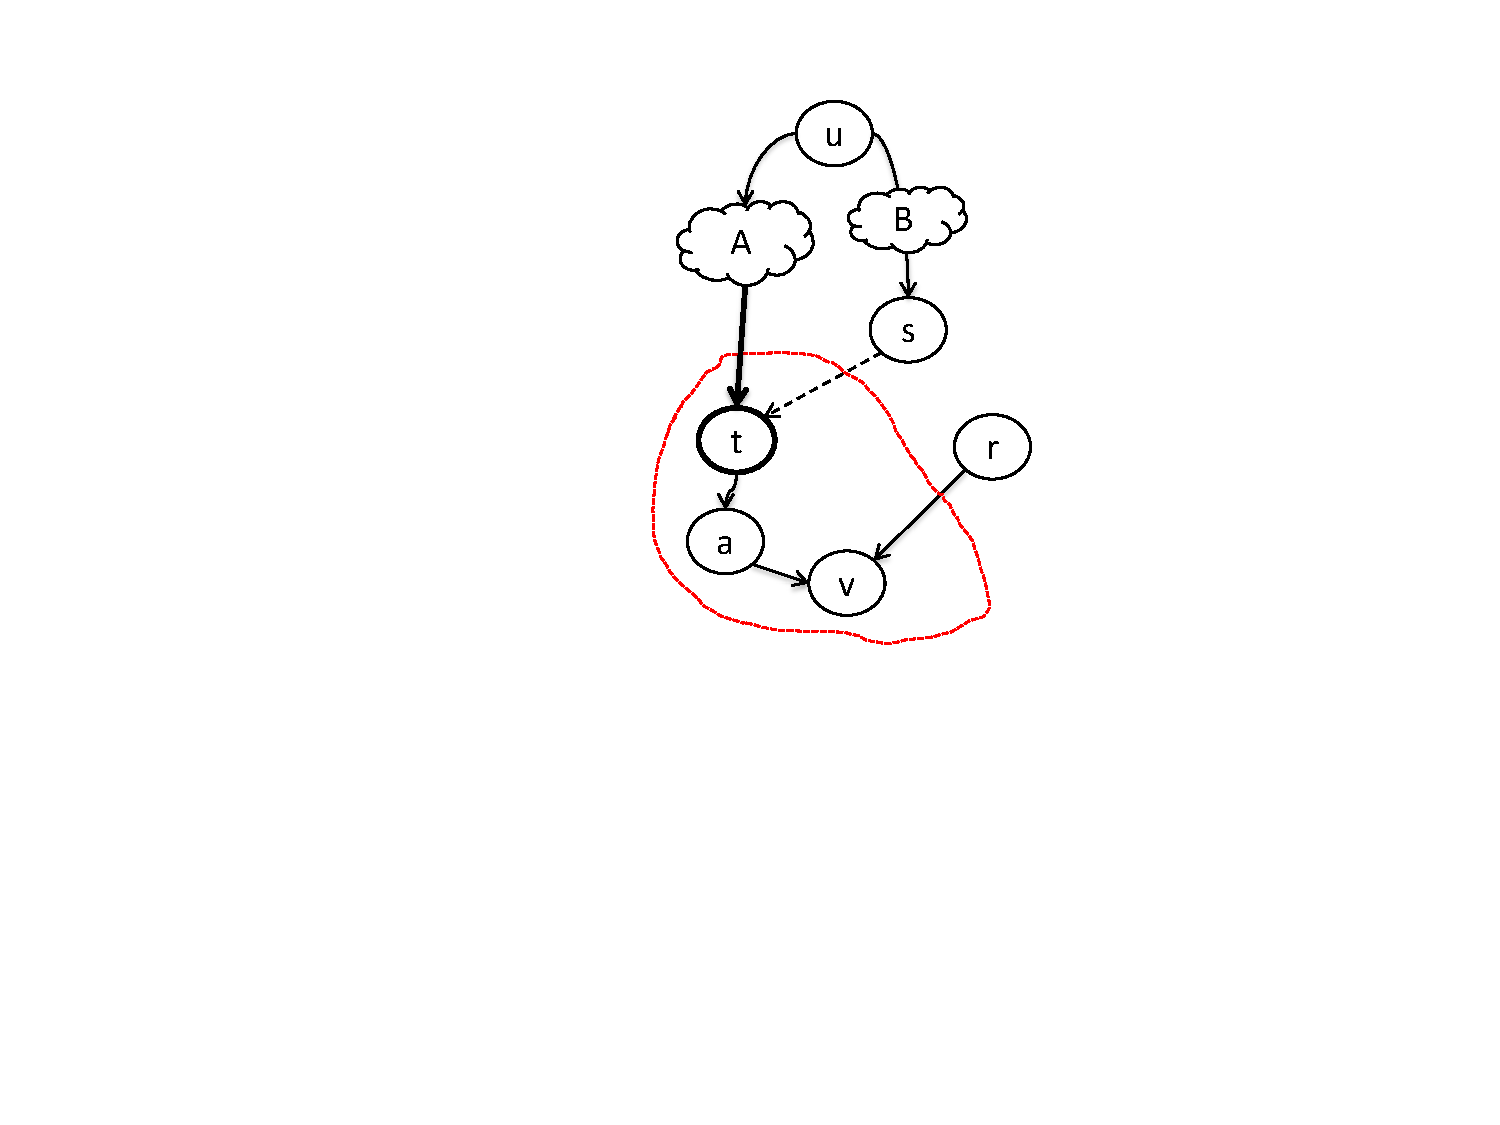
\includegraphics[width=\textwidth]{chapter3/dag_update_2.pdf}
  \caption{ Case 2}
\end{subfigure}
\begin{subfigure}{0.205\linewidth}
  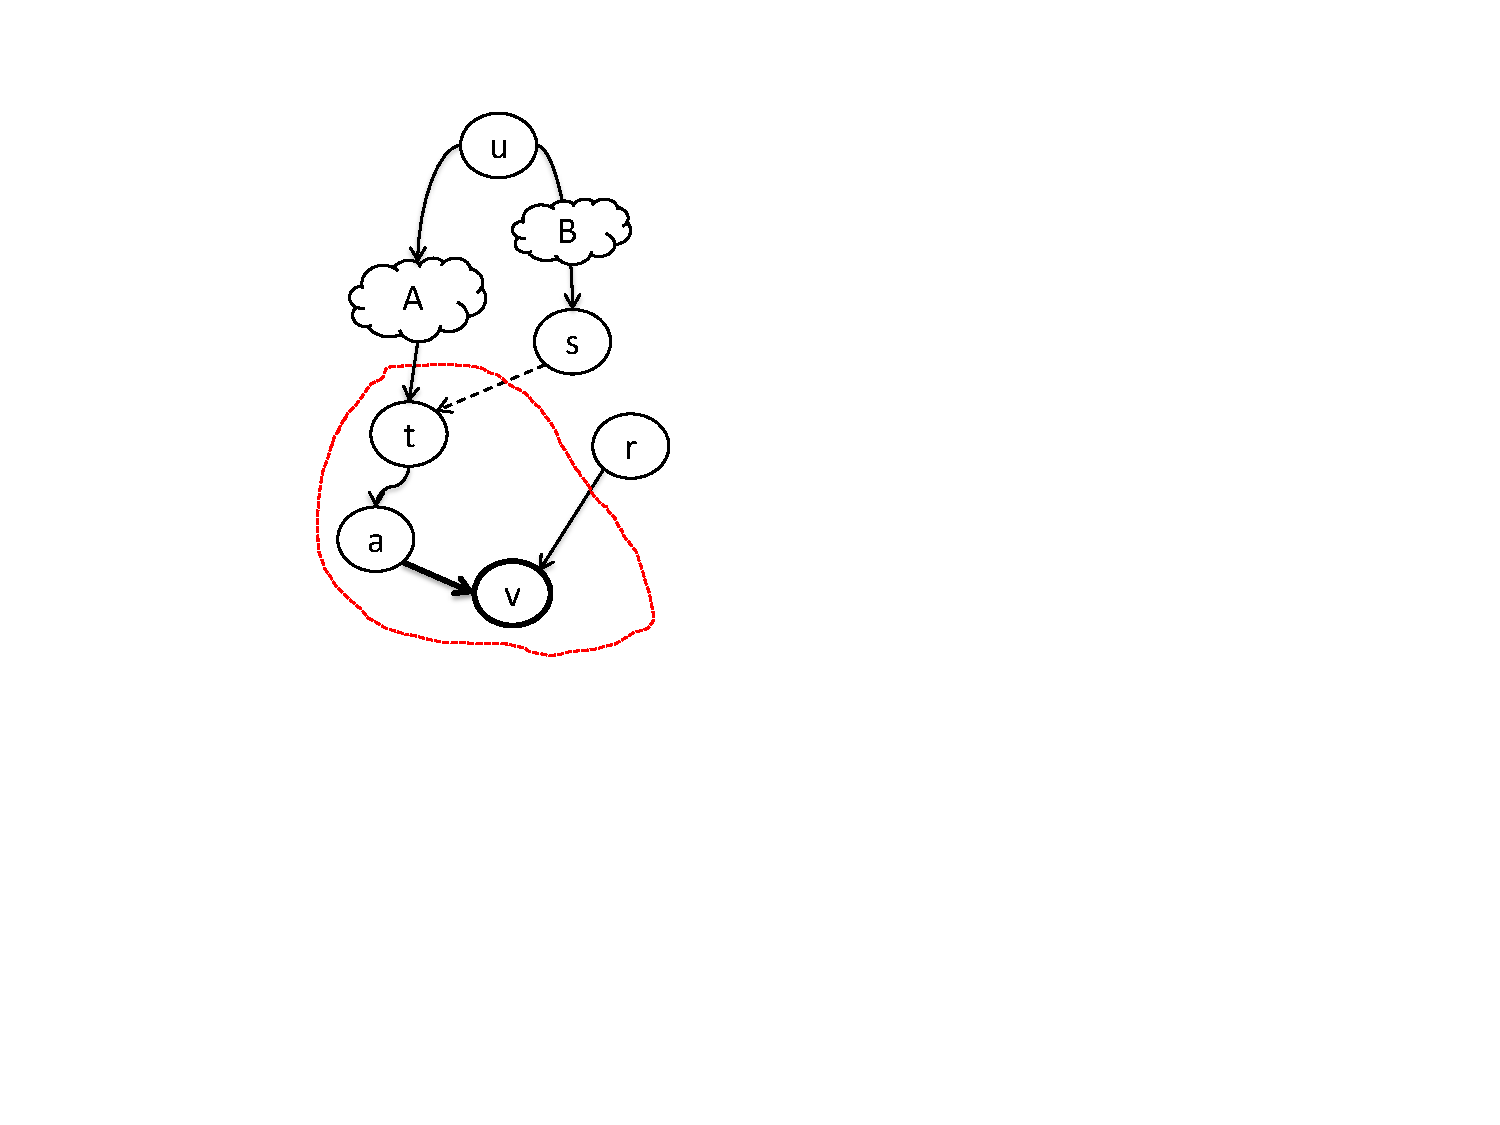
\includegraphics[width=\textwidth]{chapter3/dag_update_3.pdf}
  \caption{Case 3}
\end{subfigure}
\begin{subfigure}{0.22\linewidth}
  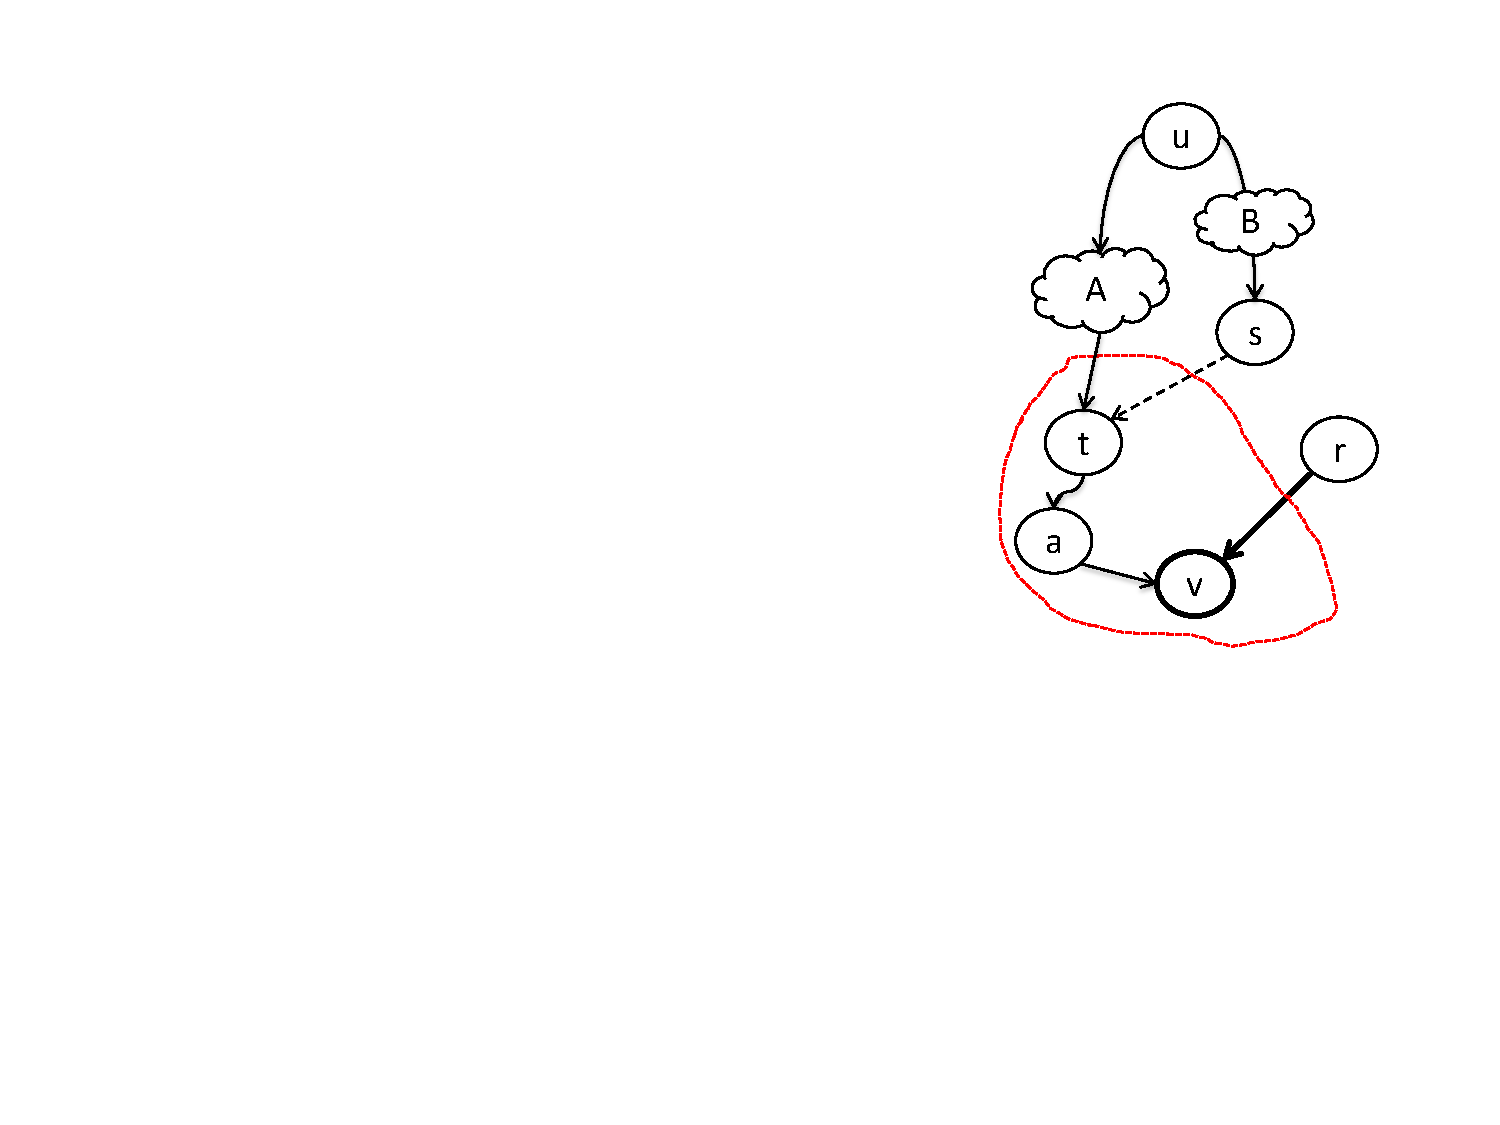
\includegraphics[width=\textwidth]{chapter3/dag_update_4.pdf}
  \caption{Case 4}
\end{subfigure}
\caption{Updates on \emph{I-Index}. Cloud shape indicate the nodes in the subgraph between the endpoint nodes. The dashed circle indicate the affected range of updates. The bold arrow indicates the $PID$ field \emph{I-Index}}
\label{fig:dag_update}
\end{figure*}
